We start with a simple example of confirmatory factor analysis, using
the \texttt{cfa()} function, which is a user-friendly function for
fitting CFA models. The lavaan package contains a built-in dataset
called \texttt{HolzingerSwineford1939}. See the help page for this
dataset by typing

\begin{verbatim}
?HolzingerSwineford1939
\end{verbatim}

at the R prompt. This is a `classic' dataset that is used in many papers
and books on Structural Equation Modeling (SEM), including some manuals
of commercial SEM software packages. The data consists of mental ability
test scores of seventh- and eighth-grade children from two different
schools (Pasteur and Grant-White). In our version of the dataset, only 9
out of the original 26 tests are included. A CFA model that is often
proposed for these 9 variables consists of three latent variables (or
factors), each with three indicators:

\begin{itemize}
\itemsep1pt\parskip0pt\parsep0pt
\item
  a \emph{visual} factor measured by 3 variables: \texttt{x1},
  \texttt{x2} and \texttt{x3}
\item
  a \emph{textual} factor measured by 3 variables: \texttt{x4},
  \texttt{x5} and \texttt{x6}
\item
  a \emph{speed} factor measured by 3 variables: \texttt{x7},
  \texttt{x8} and \texttt{x9}
\end{itemize}

The figure below contains a graphical representation of the three-factor
model.

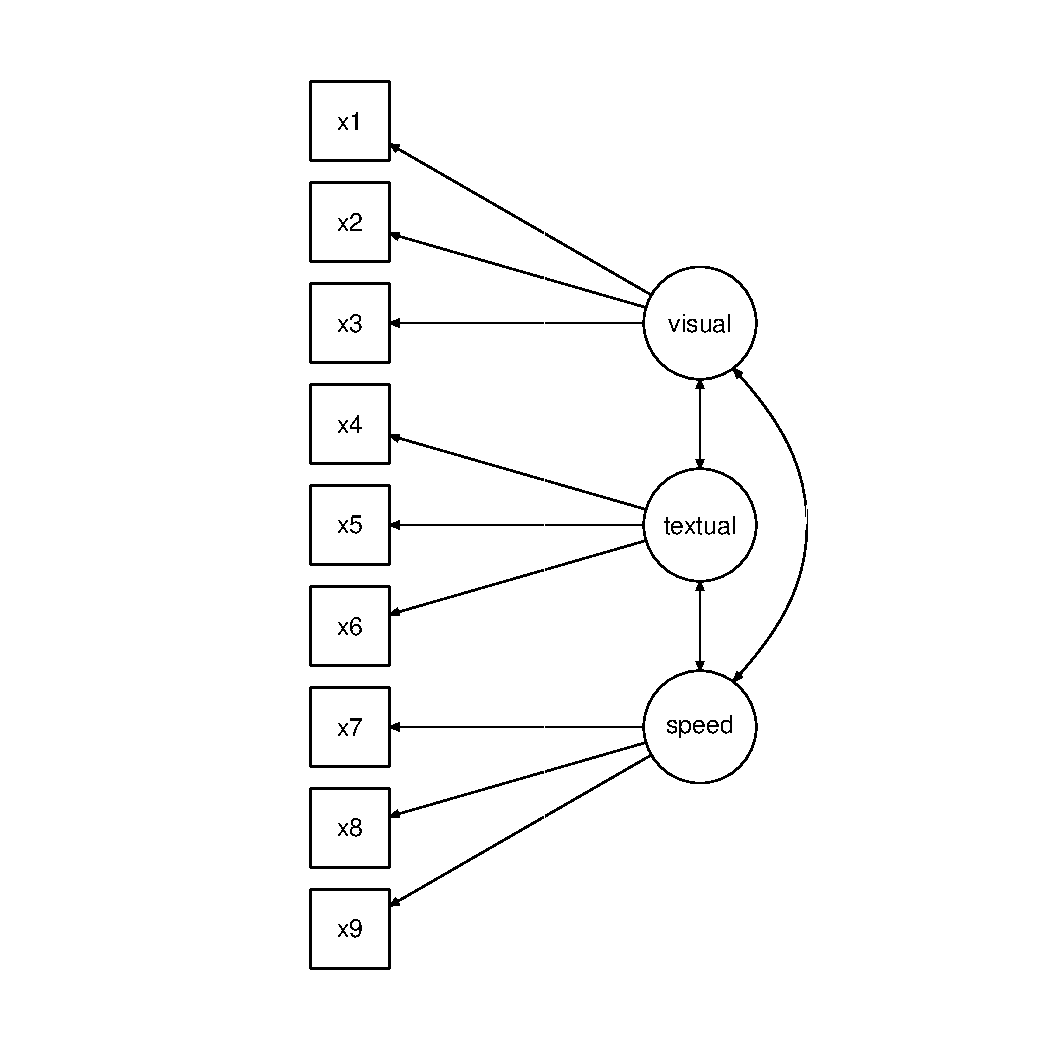
\includegraphics{figure/cfa.pdf}

The corresponding lavaan syntax for specifying this model is as follows:

\begin{verbatim}
 visual =~ x1 + x2 + x3
textual =~ x4 + x5 + x6
  speed =~ x7 + x8 + x9
\end{verbatim}

In this example, the model syntax only contains three `latent variable
definitions'. Each formula has the following format:

\begin{verbatim}
latent variable =~ indicator1 + indicator2 + indicator3
\end{verbatim}

We call these expressions \emph{latent variable definitions} because
they define how the latent variables are `manifested by' a set of
observed (or manifest) variables, often called `indicators'. Note that
the special ``\texttt{=\textasciitilde{}"} operator in the middle
consists of a sign (''\texttt{=}``) character and a tilde
(\texttt{"\textasciitilde{}"}) character next to each other. The reason
why this model syntax is so short, is that behind the scenes, the
function will take care of several things. First, by default, the factor
loading of the first indicator of a latent variable is fixed to 1,
thereby fixing the scale of the latent variable. Second, residual
variances are added automatically. And third, all exogenous latent
variables are correlated by default. This way, the model syntax can be
kept concise. On the other hand, the user remains in control, since all
this `default' behavior can be overriden and/or switched off.

We can enter the model syntax using the single quotes:

\begin{Shaded}
\begin{Highlighting}[]
\NormalTok{HS.model <-}\StringTok{ ' visual  =~ x1 + x2 + x3 }
\StringTok{              textual =~ x4 + x5 + x6}
\StringTok{              speed   =~ x7 + x8 + x9 '}
\end{Highlighting}
\end{Shaded}

We can now fit the model as follows:

\begin{Shaded}
\begin{Highlighting}[]
\NormalTok{fit <-}\StringTok{ }\KeywordTok{cfa}\NormalTok{(HS.model, }\DataTypeTok{data =} \NormalTok{HolzingerSwineford1939)}
\end{Highlighting}
\end{Shaded}

The \texttt{cfa()} function is a dedicated function for fitting
confirmatory factor analysis models. The first argument is the
user-specified model. The second argument is the dataset that contains
the observed variables. Once the model has been fitted, the
\texttt{summary()} function provides a nice summary of the fitted model:

\begin{Shaded}
\begin{Highlighting}[]
\KeywordTok{summary}\NormalTok{(fit, }\DataTypeTok{fit.measures =} \OtherTok{TRUE}\NormalTok{)}
\end{Highlighting}
\end{Shaded}

The output should look familiar to users of other SEM software. If you
find it confusing or esthetically unpleasing, please let us know, and we
will try to improve it.

\begin{verbatim}
lavaan (0.5-13) converged normally after  41 iterations

  Number of observations                           301

  Estimator                                         ML
  Minimum Function Test Statistic               85.306
  Degrees of freedom                                24
  P-value (Chi-square)                           0.000

Model test baseline model:

  Minimum Function Test Statistic              918.852
  Degrees of freedom                                36
  P-value                                        0.000

Full model versus baseline model:

  Comparative Fit Index (CFI)                    0.931
  Tucker-Lewis Index (TLI)                       0.896

Loglikelihood and Information Criteria:

  Loglikelihood user model (H0)              -3737.745
  Loglikelihood unrestricted model (H1)      -3695.092

  Number of free parameters                         21
  Akaike (AIC)                                7517.490
  Bayesian (BIC)                              7595.339
  Sample-size adjusted Bayesian (BIC)         7528.739

Root Mean Square Error of Approximation:

  RMSEA                                          0.092
  90 Percent Confidence Interval          0.071  0.114
  P-value RMSEA <= 0.05                          0.001

Standardized Root Mean Square Residual:

  SRMR                                           0.065

Parameter estimates:

  Information                                 Expected
  Standard Errors                             Standard

                   Estimate  Std.err  Z-value  P(>|z|)
Latent variables:
  visual =~
    x1                1.000
    x2                0.553    0.100    5.554    0.000
    x3                0.729    0.109    6.685    0.000
  textual =~
    x4                1.000
    x5                1.113    0.065   17.014    0.000
    x6                0.926    0.055   16.703    0.000
  speed =~
    x7                1.000
    x8                1.180    0.165    7.152    0.000
    x9                1.082    0.151    7.155    0.000

Covariances:
  visual ~~
    textual           0.408    0.074    5.552    0.000
    speed             0.262    0.056    4.660    0.000
  textual ~~
    speed             0.173    0.049    3.518    0.000

Variances:
    x1                0.549    0.114
    x2                1.134    0.102
    x3                0.844    0.091
    x4                0.371    0.048
    x5                0.446    0.058
    x6                0.356    0.043
    x7                0.799    0.081
    x8                0.488    0.074
    x9                0.566    0.071
    visual            0.809    0.145
    textual           0.979    0.112
    speed             0.384    0.086
\end{verbatim}

The output consists of three parts. The first six lines are called
\emph{the header}. The header contains the following information:

\begin{itemize}
\itemsep1pt\parskip0pt\parsep0pt
\item
  the lavaan version number
\item
  did lavaan converge normally or not, and how many iterations were
  needed
\item
  the number of observations that were effectively used in the analysis
\item
  the estimator that was used to obtain the parameter values (here:
  \texttt{ML})
\item
  the model test statistic, the degrees of freedom, and a corresponding
  p-value
\end{itemize}

The next section contains additional fit measures, and is only shown
because we use the optional argument \texttt{fit.measures = TRUE}. It
starts with the line \texttt{Model test baseline model} and ends with
the value for the \texttt{SRMR}. The last section contains the parameter
estimates. It starts with information about the standard errors (if the
information matrix is expected or observed, and if the standard errors
are standard, robust, or based on the bootstrap). Then, it tabulates all
free (and fixed) parameters that were included in the model. Typically,
first the latent variables are shown, followed by covariances and
(residual) variances. The first column (\texttt{Estimate}) contains the
(estimated or fixed) parameter value for each model parameter; the
second column (\texttt{Std.err}) contains the standard error for each
estimated parameter; the third column (\texttt{Z-value}) contains the
Wald statistic (which is simply obtained by dividing the parameter value
by its standard error), and the last column
(\texttt{P(\textgreater{}\textbar{}z\textbar{})}) contains the p-value
for testing the null hypothesis that the parameter equals zero in the
population.

To wrap up this first example, we summarize the complete code that was
needed to fit this three-factor model:

\begin{Shaded}
\begin{Highlighting}[]
\CommentTok{# load the lavaan package (only needed once per session)}
\KeywordTok{library}\NormalTok{(lavaan)}

\CommentTok{# specify the model}
\NormalTok{HS.model <-}\StringTok{ ' visual  =~ x1 + x2 + x3      }
\StringTok{              textual =~ x4 + x5 + x6}
\StringTok{              speed   =~ x7 + x8 + x9 '}

\CommentTok{# fit the model}
\NormalTok{fit <-}\StringTok{ }\KeywordTok{cfa}\NormalTok{(HS.model, }\DataTypeTok{data=}\NormalTok{HolzingerSwineford1939)}

\CommentTok{# display summary output}
\KeywordTok{summary}\NormalTok{(fit, }\DataTypeTok{fit.measures=}\OtherTok{TRUE}\NormalTok{)}
\end{Highlighting}
\end{Shaded}

Simply copying this code and pasting it in R should work. The syntax
illustrates the typical workflow in the lavaan package:

\begin{enumerate}
\def\labelenumi{\arabic{enumi}.}
\item
  Specify your model using the lavaan model syntax. In this example,
  only \emph{latent variable definitions} have been used. In the
  following examples, other formula types will be used.
\item
  Fit the model. This requires a dataset containing the observed
  variables (or alternatively the sample covariance matrix and the
  number of observations). In this example, we have used the
  \texttt{cfa()} function. Other funcions in the lavaan package are
  \texttt{sem()} and \texttt{growth()} for fitting full structural
  equation models and growth curve models respectively. All three
  functions are so-called user-friendly functions, in the sense that
  they take care of many details automatically, so we can keep the model
  syntax simple and concise. If you wish to fit non-standard models or
  if you don't like the idea that things are done for you automatically,
  you can use the lower-level function \texttt{lavaan()} instead, where
  you have full control.
\item
  Extract information from the fitted model. This can be a long verbose
  summary, or it can be a single number only (say, the RMSEA value). In
  the spirit of R, you only get what you asked for. We try to not print
  out unnecessary information that you would ignore anyway.
\end{enumerate}
